\section{Welke kabel is gekozen en waarom?}

Om de optimale kabel te kiezen is het bepalen van de stromen die door de kabel zullen lopen belangrijk. De stromen die door de kabels zullen stromen hangen af van meerdere factoren. Ten eerste is het aantal turbines van belang. In het windpark zijn, zoals in het vorige hoofdstuk aangegeven, de turbines met groepen van vier, drie of één via een inter array kabel verbonden met het TenneT-station. Het totale werkelijk vermogen P wat dan door de kabel zal moeten, verschilt dus van 72MW tot 18MW. Om de stromen te kunnen berekenen is in eerste instantie een kabel gekozen waarvan de current rating wordt gebruikt om de rest van de gegevens te bepalen. Hieronder zijn de formules te zien, de berekeningen met getallen zijn ter voorbeeld ingevuld voor de configuratie van 4 turbines, aangezien dit de meest voorkomende hoeveelheid turbines per array is.   

\begin{equation} \label{eq:Pfase}
P\textsubscript{fase} = \frac{P\textsubscript{turbine} \times N\textsubscript{turbines}}{3} = \frac{18.000.000 \times 4}{3} = 24.000.000W
\end{equation} 

In een ster configuratie 3 fase kabel geldt: 

I\textsubscript{fase} = I\textsubscript{lijn}

Door eerst een kabel te kiezen die verwacht wordt geschikt te zijn, kan met de current rating van deze kabel worden bepaald dat I\textsubscript{lijn} en I\textsubscript{fase} beiden gelijk zijn aan 775A. Met dit bekend en de bekende lijnspanning van 66kV, kan de fasespanning, het schijnbaar vermogen S en daarna de arbeidsfactor berekend worden zoals gedaan in formules \ref{eq:Ufase}, \ref{eq:S} en \ref{eq:Arbeidfactor}.\cite{Technische_Aspecten_Presentatie}\cite{Three_phase_calculator}

\begin{equation} \label{eq:Ufase}
U\textsubscript{fase} = \frac{U\textsubscript{lijn}}{\sqrt{3}} = \frac{66.000}{\sqrt{3}} = 38.105V
\end{equation} 

\begin{equation} \label{eq:S}
S = 3 \times I\textsubscript{fase} \times U\textsubscript{fase} = 3 \times 775 \times 38.105 = 88.594.399VA
\end{equation}

Met S en P kan vervolgens de arbeidsfactor worden berekend met: 

\begin{equation} \label{eq:Arbeidfactor}
Arbeidsfactor = \frac{P}{S} = \frac{72.000.000}{88.594.399} = 0,81
\end{equation}

Aangezien nu de current rating van de kabel is gebruikt, welke in werkelijkheid niet zo hoog zal zijn, valt te stellen dat de arbeidsfactor in werkelijkheid wat hoger is. Daarom wordt uitgegaan van een realistische arbeidsfactor van 0,85. Hiermee kunnen vervolgens de werkelijke stromen door de kabels berekend worden met de formules \ref{eq:Swerk} en \ref{eq:Ifasewerk}. 

\begin{equation} \label{eq:Swerk}
S\textsubscript{werk} = \frac{P}{Arbeidsfactor} = \frac{72.000.000}{0,85} = 84.705.882VA
\end{equation}

\begin{equation} \label{eq:Ifasewerk}
I\textsubscript{fase, werk} = \frac{S\textsubscript{werk}/3}{U\textsubscript{fase}} = \frac{84.705.882/3}{38.105} = 740,98A
\end{equation}

Met al deze gegevens kunnen vervolgens het blind vermogen Q en het vermogensverlies P\textsubscript{verlies} berekend worden zoals te zien in formule \ref{eq:Q} en \ref{eq:Pverlies}.

\begin{equation} \label{eq:Q}
Q = \sqrt{S\textsubscript{tot, werk}^2 - (P\textsubscript{turbine} \times N)^2} = \sqrt{84.705.882^2 - (18.000.000 \times 4)^2} = 44.621.592var
\end{equation}

\begin{equation} \label{eq:Pverlies}
P\textsubscript{verlies} = I\textsubscript{tot, werk}^2 \times R = 740,98^2 \times 0,137 = 75.307W
\end{equation}

Bij het vermogensverlies speelt de weerstand R uiteraard een grote rol. Deze verschilt per kabel, omdat het afhankelijk is van de lengte. De weerstand is voor elke kabel los berekend (zie tabel \ref{tab:Kavel VI - aangevulde data} en \ref{tab:Kavel VII - aangevulde data}) en gebruikt in de berekeningen.


\begin{table}[]
\resizebox{\textwidth}{!}{%
\begin{tabular}{|llllllllllllll|}
\hline
\rowcolor[HTML]{A5A5A5} 
\multicolumn{14}{|c|}{\cellcolor[HTML]{A5A5A5}{\color[HTML]{333333} \textbf{Kavel VI}}} \\ \hline
\rowcolor[HTML]{A5A5A5} 
\multicolumn{1}{|l|}{\cellcolor[HTML]{A5A5A5}{\color[HTML]{333333} \textbf{Kabel}}} &
  \multicolumn{1}{l|}{\cellcolor[HTML]{A5A5A5}{\color[HTML]{333333} \textbf{1}}} &
  \multicolumn{1}{l|}{\cellcolor[HTML]{A5A5A5}{\color[HTML]{333333} \textbf{2}}} &
  \multicolumn{1}{l|}{\cellcolor[HTML]{A5A5A5}{\color[HTML]{333333} \textbf{3}}} &
  \multicolumn{1}{l|}{\cellcolor[HTML]{A5A5A5}{\color[HTML]{333333} \textbf{4}}} &
  \multicolumn{1}{l|}{\cellcolor[HTML]{A5A5A5}{\color[HTML]{333333} \textbf{5}}} &
  \multicolumn{1}{l|}{\cellcolor[HTML]{A5A5A5}{\color[HTML]{333333} \textbf{6}}} &
  \multicolumn{1}{l|}{\cellcolor[HTML]{A5A5A5}{\color[HTML]{333333} \textbf{7}}} &
  \multicolumn{1}{l|}{\cellcolor[HTML]{A5A5A5}{\color[HTML]{333333} \textbf{8}}} &
  \multicolumn{1}{l|}{\cellcolor[HTML]{A5A5A5}{\color[HTML]{333333} \textbf{9}}} &
  \multicolumn{1}{l|}{\cellcolor[HTML]{A5A5A5}{\color[HTML]{333333} \textbf{10}}} &
  \multicolumn{1}{l|}{\cellcolor[HTML]{A5A5A5}{\color[HTML]{333333} \textbf{11}}} &
  \multicolumn{1}{l|}{\cellcolor[HTML]{A5A5A5}{\color[HTML]{333333} \textbf{12}}} &
  {\color[HTML]{333333} \textbf{13}} \\ \hline
\rowcolor[HTML]{FFFFFF} 
\multicolumn{1}{|l|}{\cellcolor[HTML]{A5A5A5}{\color[HTML]{333333} \textbf{Aantal turbines}}} &
  \multicolumn{1}{c|}{\cellcolor[HTML]{FFFFFF}{\color[HTML]{333333} 4}} &
  \multicolumn{1}{l|}{\cellcolor[HTML]{FFFFFF}{\color[HTML]{333333} 4}} &
  \multicolumn{1}{l|}{\cellcolor[HTML]{FFFFFF}{\color[HTML]{333333} 1}} &
  \multicolumn{1}{l|}{\cellcolor[HTML]{FFFFFF}{\color[HTML]{333333} 4}} &
  \multicolumn{1}{l|}{\cellcolor[HTML]{FFFFFF}{\color[HTML]{333333} 4}} &
  \multicolumn{1}{l|}{\cellcolor[HTML]{FFFFFF}{\color[HTML]{333333} 4}} &
  \multicolumn{1}{l|}{\cellcolor[HTML]{FFFFFF}{\color[HTML]{333333} 3}} &
  \multicolumn{1}{l|}{\cellcolor[HTML]{FFFFFF}{\color[HTML]{333333} 4}} &
  \multicolumn{1}{l|}{\cellcolor[HTML]{FFFFFF}{\color[HTML]{333333} 4}} &
  \multicolumn{1}{l|}{\cellcolor[HTML]{FFFFFF}{\color[HTML]{333333} 4}} &
  \multicolumn{1}{l|}{\cellcolor[HTML]{FFFFFF}{\color[HTML]{333333} 4}} &
  \multicolumn{1}{l|}{\cellcolor[HTML]{FFFFFF}{\color[HTML]{333333} 4}} &
  {\color[HTML]{333333} 4} \\ \hline
\rowcolor[HTML]{DBDBDB} 
\multicolumn{1}{|l|}{\cellcolor[HTML]{A5A5A5}{\color[HTML]{333333} \textbf{Weerstand {[}\(\Omega\){]}}}} & 
  \multicolumn{1}{l|}{\cellcolor[HTML]{DBDBDB}{\color[HTML]{333333} 0,117}} &
  \multicolumn{1}{l|}{\cellcolor[HTML]{DBDBDB}{\color[HTML]{333333} 0,116}} &
  \multicolumn{1}{l|}{\cellcolor[HTML]{DBDBDB}{\color[HTML]{333333} 0,028}} &
  \multicolumn{1}{l|}{\cellcolor[HTML]{DBDBDB}{\color[HTML]{333333} 0,298}} &
  \multicolumn{1}{l|}{\cellcolor[HTML]{DBDBDB}{\color[HTML]{333333} 0,180}} &
  \multicolumn{1}{l|}{\cellcolor[HTML]{DBDBDB}{\color[HTML]{333333} 0,306}} &
  \multicolumn{1}{l|}{\cellcolor[HTML]{DBDBDB}{\color[HTML]{333333} 0,079}} &
  \multicolumn{1}{l|}{\cellcolor[HTML]{DBDBDB}{\color[HTML]{333333} 0,157}} &
  \multicolumn{1}{l|}{\cellcolor[HTML]{DBDBDB}{\color[HTML]{333333} 0,176}} &
  \multicolumn{1}{l|}{\cellcolor[HTML]{DBDBDB}{\color[HTML]{333333} 0,239}} &
  \multicolumn{1}{l|}{\cellcolor[HTML]{DBDBDB}{\color[HTML]{333333} 0,150}} &
  \multicolumn{1}{l|}{\cellcolor[HTML]{DBDBDB}{\color[HTML]{333333} 0,081}} &
  {\color[HTML]{333333} 0,129} \\ \hline
\rowcolor[HTML]{FFFFFF} 
\multicolumn{1}{|l|}{\cellcolor[HTML]{A5A5A5}{\color[HTML]{333333} \textbf{Stroom fase (I) {[}A{]}}}} &
  \multicolumn{1}{l|}{\cellcolor[HTML]{FFFFFF}{\color[HTML]{333333} 740,98}} &
  \multicolumn{1}{l|}{\cellcolor[HTML]{FFFFFF}{\color[HTML]{333333} 740,98}} &
  \multicolumn{1}{l|}{\cellcolor[HTML]{FFFFFF}{\color[HTML]{333333} 185,25}} &
  \multicolumn{1}{l|}{\cellcolor[HTML]{FFFFFF}{\color[HTML]{333333} 740,98}} &
  \multicolumn{1}{l|}{\cellcolor[HTML]{FFFFFF}{\color[HTML]{333333} 740,98}} &
  \multicolumn{1}{l|}{\cellcolor[HTML]{FFFFFF}{\color[HTML]{333333} 740,98}} &
  \multicolumn{1}{l|}{\cellcolor[HTML]{FFFFFF}{\color[HTML]{333333} 555,74}} &
  \multicolumn{1}{l|}{\cellcolor[HTML]{FFFFFF}{\color[HTML]{333333} 740,98}} &
  \multicolumn{1}{l|}{\cellcolor[HTML]{FFFFFF}{\color[HTML]{333333} 740,98}} &
  \multicolumn{1}{l|}{\cellcolor[HTML]{FFFFFF}{\color[HTML]{333333} 740,98}} &
  \multicolumn{1}{l|}{\cellcolor[HTML]{FFFFFF}{\color[HTML]{333333} 740,98}} &
  \multicolumn{1}{l|}{\cellcolor[HTML]{FFFFFF}{\color[HTML]{333333} 740,98}} &
  {\color[HTML]{333333} 740,98} \\ \hline
\rowcolor[HTML]{DBDBDB} 
\multicolumn{1}{|l|}{\cellcolor[HTML]{A5A5A5}{\color[HTML]{333333} \textbf{Stroom totaal (I) {[}A{]}}}} &
  \multicolumn{1}{l|}{\cellcolor[HTML]{DBDBDB}{\color[HTML]{333333} 740,98}} &
  \multicolumn{1}{l|}{\cellcolor[HTML]{DBDBDB}{\color[HTML]{333333} 740,98}} &
  \multicolumn{1}{l|}{\cellcolor[HTML]{DBDBDB}{\color[HTML]{333333} 185,25}} &
  \multicolumn{1}{l|}{\cellcolor[HTML]{DBDBDB}{\color[HTML]{333333} 740,98}} &
  \multicolumn{1}{l|}{\cellcolor[HTML]{DBDBDB}{\color[HTML]{333333} 740,98}} &
  \multicolumn{1}{l|}{\cellcolor[HTML]{DBDBDB}{\color[HTML]{333333} 740,98}} &
  \multicolumn{1}{l|}{\cellcolor[HTML]{DBDBDB}{\color[HTML]{333333} 555,74}} &
  \multicolumn{1}{l|}{\cellcolor[HTML]{DBDBDB}{\color[HTML]{333333} 740,98}} &
  \multicolumn{1}{l|}{\cellcolor[HTML]{DBDBDB}{\color[HTML]{333333} 740,98}} &
  \multicolumn{1}{l|}{\cellcolor[HTML]{DBDBDB}{\color[HTML]{333333} 740,98}} &
  \multicolumn{1}{l|}{\cellcolor[HTML]{DBDBDB}{\color[HTML]{333333} 740,98}} &
  \multicolumn{1}{l|}{\cellcolor[HTML]{DBDBDB}{\color[HTML]{333333} 740,98}} &
  {\color[HTML]{333333} 740,98} \\ \hline
\rowcolor[HTML]{FFFFFF} 
\multicolumn{1}{|l|}{\cellcolor[HTML]{A5A5A5}{\color[HTML]{333333} \textbf{Pfase {[}MW{]}}}} &
  \multicolumn{1}{l|}{\cellcolor[HTML]{FFFFFF}{\color[HTML]{333333} 24}} &
  \multicolumn{1}{l|}{\cellcolor[HTML]{FFFFFF}{\color[HTML]{333333} 24}} &
  \multicolumn{1}{l|}{\cellcolor[HTML]{FFFFFF}{\color[HTML]{333333} 6}} &
  \multicolumn{1}{l|}{\cellcolor[HTML]{FFFFFF}{\color[HTML]{333333} 24}} &
  \multicolumn{1}{l|}{\cellcolor[HTML]{FFFFFF}{\color[HTML]{333333} 24}} &
  \multicolumn{1}{l|}{\cellcolor[HTML]{FFFFFF}{\color[HTML]{333333} 24}} &
  \multicolumn{1}{l|}{\cellcolor[HTML]{FFFFFF}{\color[HTML]{333333} 18}} &
  \multicolumn{1}{l|}{\cellcolor[HTML]{FFFFFF}{\color[HTML]{333333} 24}} &
  \multicolumn{1}{l|}{\cellcolor[HTML]{FFFFFF}{\color[HTML]{333333} 24}} &
  \multicolumn{1}{l|}{\cellcolor[HTML]{FFFFFF}{\color[HTML]{333333} 24}} &
  \multicolumn{1}{l|}{\cellcolor[HTML]{FFFFFF}{\color[HTML]{333333} 24}} &
  \multicolumn{1}{l|}{\cellcolor[HTML]{FFFFFF}{\color[HTML]{333333} 24}} &
  {\color[HTML]{333333} 24} \\ \hline
\rowcolor[HTML]{DBDBDB} 
\multicolumn{1}{|l|}{\cellcolor[HTML]{A5A5A5}{\color[HTML]{333333} \textbf{Ptotaal   {[}MW{]}}}} &
  \multicolumn{1}{l|}{\cellcolor[HTML]{DBDBDB}{\color[HTML]{333333} 72}} &
  \multicolumn{1}{l|}{\cellcolor[HTML]{DBDBDB}{\color[HTML]{333333} 72}} &
  \multicolumn{1}{l|}{\cellcolor[HTML]{DBDBDB}{\color[HTML]{333333} 18}} &
  \multicolumn{1}{l|}{\cellcolor[HTML]{DBDBDB}{\color[HTML]{333333} 72}} &
  \multicolumn{1}{l|}{\cellcolor[HTML]{DBDBDB}{\color[HTML]{333333} 72}} &
  \multicolumn{1}{l|}{\cellcolor[HTML]{DBDBDB}{\color[HTML]{333333} 72}} &
  \multicolumn{1}{l|}{\cellcolor[HTML]{DBDBDB}{\color[HTML]{333333} 54}} &
  \multicolumn{1}{l|}{\cellcolor[HTML]{DBDBDB}{\color[HTML]{333333} 72}} &
  \multicolumn{1}{l|}{\cellcolor[HTML]{DBDBDB}{\color[HTML]{333333} 72}} &
  \multicolumn{1}{l|}{\cellcolor[HTML]{DBDBDB}{\color[HTML]{333333} 72}} &
  \multicolumn{1}{l|}{\cellcolor[HTML]{DBDBDB}{\color[HTML]{333333} 72}} &
  \multicolumn{1}{l|}{\cellcolor[HTML]{DBDBDB}{\color[HTML]{333333} 72}} &
  {\color[HTML]{333333} 72} \\ \hline
\rowcolor[HTML]{FFFFFF} 
\multicolumn{1}{|l|}{\cellcolor[HTML]{A5A5A5}{\color[HTML]{333333} \textbf{Swerk {[}MVA{]}}}} &
  \multicolumn{1}{l|}{\cellcolor[HTML]{FFFFFF}{\color[HTML]{333333} 84705,9}} &
  \multicolumn{1}{l|}{\cellcolor[HTML]{FFFFFF}{\color[HTML]{333333} 84705,9}} &
  \multicolumn{1}{l|}{\cellcolor[HTML]{FFFFFF}{\color[HTML]{333333} 21176,6}} &
  \multicolumn{1}{l|}{\cellcolor[HTML]{FFFFFF}{\color[HTML]{333333} 84705,9}} &
  \multicolumn{1}{l|}{\cellcolor[HTML]{FFFFFF}{\color[HTML]{333333} 84705,9}} &
  \multicolumn{1}{l|}{\cellcolor[HTML]{FFFFFF}{\color[HTML]{333333} 84705,9}} &
  \multicolumn{1}{l|}{\cellcolor[HTML]{FFFFFF}{\color[HTML]{333333} 63529,4}} &
  \multicolumn{1}{l|}{\cellcolor[HTML]{FFFFFF}{\color[HTML]{333333} 84705,9}} &
  \multicolumn{1}{l|}{\cellcolor[HTML]{FFFFFF}{\color[HTML]{333333} 84705,9}} &
  \multicolumn{1}{l|}{\cellcolor[HTML]{FFFFFF}{\color[HTML]{333333} 84705,9}} &
  \multicolumn{1}{l|}{\cellcolor[HTML]{FFFFFF}{\color[HTML]{333333} 84705,9}} &
  \multicolumn{1}{l|}{\cellcolor[HTML]{FFFFFF}{\color[HTML]{333333} 84705,9}} &
  \cellcolor[HTML]{FFFFFF}{\color[HTML]{333333} 84705,9} \\ \hline
\rowcolor[HTML]{DBDBDB} 
\multicolumn{1}{|l|}{\cellcolor[HTML]{A5A5A5}{\color[HTML]{333333} \textbf{Q {[}kvar{]}}}} &
  \multicolumn{1}{l|}{\cellcolor[HTML]{DBDBDB}{\color[HTML]{333333} 44621,6}} &
  \multicolumn{1}{l|}{\cellcolor[HTML]{DBDBDB}{\color[HTML]{333333} 44621,6}} &
  \multicolumn{1}{l|}{\cellcolor[HTML]{DBDBDB}{\color[HTML]{333333} 11155,4}} &
  \multicolumn{1}{l|}{\cellcolor[HTML]{DBDBDB}{\color[HTML]{333333} 44621,6}} &
  \multicolumn{1}{l|}{\cellcolor[HTML]{DBDBDB}{\color[HTML]{333333} 44621,6}} &
  \multicolumn{1}{l|}{\cellcolor[HTML]{DBDBDB}{\color[HTML]{333333} 44621,6}} &
  \multicolumn{1}{l|}{\cellcolor[HTML]{DBDBDB}{\color[HTML]{333333} 33466,2}} &
  \multicolumn{1}{l|}{\cellcolor[HTML]{DBDBDB}{\color[HTML]{333333} 44621,6}} &
  \multicolumn{1}{l|}{\cellcolor[HTML]{DBDBDB}{\color[HTML]{333333} 44621,6}} &
  \multicolumn{1}{l|}{\cellcolor[HTML]{DBDBDB}{\color[HTML]{333333} 44621,6}} &
  \multicolumn{1}{l|}{\cellcolor[HTML]{DBDBDB}{\color[HTML]{333333} 44621,6}} &
  \multicolumn{1}{l|}{\cellcolor[HTML]{DBDBDB}{\color[HTML]{333333} 44621,6}} &
  \cellcolor[HTML]{DBDBDB}{\color[HTML]{333333} 44621,6} \\ \hline
\rowcolor[HTML]{FFFFFF} 
\multicolumn{1}{|l|}{\cellcolor[HTML]{A5A5A5}{\color[HTML]{333333} \textbf{Pverliezen {[}W{]}}}} &
  \multicolumn{1}{l|}{\cellcolor[HTML]{FFFFFF}{\color[HTML]{333333} 64257}} &
  \multicolumn{1}{l|}{\cellcolor[HTML]{FFFFFF}{\color[HTML]{333333} 63608}} &
  \multicolumn{1}{l|}{\cellcolor[HTML]{FFFFFF}{\color[HTML]{333333} 955}} &
  \multicolumn{1}{l|}{\cellcolor[HTML]{FFFFFF}{\color[HTML]{333333} 163381}} &
  \multicolumn{1}{l|}{\cellcolor[HTML]{FFFFFF}{\color[HTML]{333333} 98896}} &
  \multicolumn{1}{l|}{\cellcolor[HTML]{FFFFFF}{\color[HTML]{333333} 168185}} &
  \multicolumn{1}{l|}{\cellcolor[HTML]{FFFFFF}{\color[HTML]{333333} 24504}} &
  \multicolumn{1}{l|}{\cellcolor[HTML]{FFFFFF}{\color[HTML]{333333} 86200}} &
  \multicolumn{1}{l|}{\cellcolor[HTML]{FFFFFF}{\color[HTML]{333333} 96493}} &
  \multicolumn{1}{l|}{\cellcolor[HTML]{FFFFFF}{\color[HTML]{333333} 131048}} &
  \multicolumn{1}{l|}{\cellcolor[HTML]{FFFFFF}{\color[HTML]{333333} 82093}} &
  \multicolumn{1}{l|}{\cellcolor[HTML]{FFFFFF}{\color[HTML]{333333} 44728}} &
  {\color[HTML]{333333} 70671} \\ \hline
\rowcolor[HTML]{DBDBDB} 
\multicolumn{1}{|l|}{\cellcolor[HTML]{A5A5A5}{\color[HTML]{333333} \textbf{Verliezen {[}\%{]}}}} &
  \multicolumn{1}{l|}{\cellcolor[HTML]{DBDBDB}{\color[HTML]{333333} 0,089\%}} &
  \multicolumn{1}{l|}{\cellcolor[HTML]{DBDBDB}{\color[HTML]{333333} 0,088\%}} &
  \multicolumn{1}{l|}{\cellcolor[HTML]{DBDBDB}{\color[HTML]{333333} 0,005\%}} &
  \multicolumn{1}{l|}{\cellcolor[HTML]{DBDBDB}{\color[HTML]{333333} 0,227\%}} &
  \multicolumn{1}{l|}{\cellcolor[HTML]{DBDBDB}{\color[HTML]{333333} 0,137\%}} &
  \multicolumn{1}{l|}{\cellcolor[HTML]{DBDBDB}{\color[HTML]{333333} 0,234\%}} &
  \multicolumn{1}{l|}{\cellcolor[HTML]{DBDBDB}{\color[HTML]{333333} 0,045\%}} &
  \multicolumn{1}{l|}{\cellcolor[HTML]{DBDBDB}{\color[HTML]{333333} 0,120\%}} &
  \multicolumn{1}{l|}{\cellcolor[HTML]{DBDBDB}{\color[HTML]{333333} 0,134\%}} &
  \multicolumn{1}{l|}{\cellcolor[HTML]{DBDBDB}{\color[HTML]{333333} 0,182\%}} &
  \multicolumn{1}{l|}{\cellcolor[HTML]{DBDBDB}{\color[HTML]{333333} 0,114\%}} &
  \multicolumn{1}{l|}{\cellcolor[HTML]{DBDBDB}{\color[HTML]{333333} 0,062\%}} &
  {\color[HTML]{333333} 0,098\%} \\ \hline
\rowcolor[HTML]{FFFFFF} 
\multicolumn{1}{|l|}{\cellcolor[HTML]{A5A5A5}{\color[HTML]{333333} \textbf{Netto vermogen {[}kW{]}}}} &
  \multicolumn{1}{l|}{\cellcolor[HTML]{FFFFFF}{\color[HTML]{333333} 71935,7}} &
  \multicolumn{1}{l|}{\cellcolor[HTML]{FFFFFF}{\color[HTML]{333333} 71936,4}} &
  \multicolumn{1}{l|}{\cellcolor[HTML]{FFFFFF}{\color[HTML]{333333} 17999,0}} &
  \multicolumn{1}{l|}{\cellcolor[HTML]{FFFFFF}{\color[HTML]{333333} 71836,6}} &
  \multicolumn{1}{l|}{\cellcolor[HTML]{FFFFFF}{\color[HTML]{333333} 71901,1}} &
  \multicolumn{1}{l|}{\cellcolor[HTML]{FFFFFF}{\color[HTML]{333333} 71831,8}} &
  \multicolumn{1}{l|}{\cellcolor[HTML]{FFFFFF}{\color[HTML]{333333} 53975,5}} &
  \multicolumn{1}{l|}{\cellcolor[HTML]{FFFFFF}{\color[HTML]{333333} 71913,8}} &
  \multicolumn{1}{l|}{\cellcolor[HTML]{FFFFFF}{\color[HTML]{333333} 71903,5}} &
  \multicolumn{1}{l|}{\cellcolor[HTML]{FFFFFF}{\color[HTML]{333333} 71869,0}} &
  \multicolumn{1}{l|}{\cellcolor[HTML]{FFFFFF}{\color[HTML]{333333} 71917,9}} &
  \multicolumn{1}{l|}{\cellcolor[HTML]{FFFFFF}{\color[HTML]{333333} 71955,3}} &
  {\color[HTML]{333333} 71929,3} \\ \hline
\end{tabular}
}
\caption{Tabel: Uitkomsten berekeningen kabels - kavel VI}
\label{tab:Kavel VI - aangevulde data}
\end{table}

\begin{table}[]
\resizebox{\textwidth}{!}{%
\begin{tabular}{|lllllllllllllll|}
\hline
\rowcolor[HTML]{A5A5A5} 
\multicolumn{15}{|c|}{\cellcolor[HTML]{A5A5A5}{\color[HTML]{333333} \textbf{Kavel VII}}} \\ \hline
\rowcolor[HTML]{A5A5A5} 
\multicolumn{1}{|l|}{\cellcolor[HTML]{A5A5A5}{\color[HTML]{333333} \textbf{Kabel}}} &
  \multicolumn{1}{l|}{\cellcolor[HTML]{A5A5A5}{\color[HTML]{333333} \textbf{1}}} &
  \multicolumn{1}{l|}{\cellcolor[HTML]{A5A5A5}{\color[HTML]{333333} \textbf{2}}} &
  \multicolumn{1}{l|}{\cellcolor[HTML]{A5A5A5}{\color[HTML]{333333} \textbf{3}}} &
  \multicolumn{1}{l|}{\cellcolor[HTML]{A5A5A5}{\color[HTML]{333333} \textbf{4}}} &
  \multicolumn{1}{l|}{\cellcolor[HTML]{A5A5A5}{\color[HTML]{333333} \textbf{5}}} &
  \multicolumn{1}{l|}{\cellcolor[HTML]{A5A5A5}{\color[HTML]{333333} \textbf{6}}} &
  \multicolumn{1}{l|}{\cellcolor[HTML]{A5A5A5}{\color[HTML]{333333} \textbf{7}}} &
  \multicolumn{1}{l|}{\cellcolor[HTML]{A5A5A5}{\color[HTML]{333333} \textbf{8}}} &
  \multicolumn{1}{l|}{\cellcolor[HTML]{A5A5A5}{\color[HTML]{333333} \textbf{9}}} &
  \multicolumn{1}{l|}{\cellcolor[HTML]{A5A5A5}{\color[HTML]{333333} \textbf{10}}} &
  \multicolumn{1}{l|}{\cellcolor[HTML]{A5A5A5}{\color[HTML]{333333} \textbf{11}}} &
  \multicolumn{1}{l|}{\cellcolor[HTML]{A5A5A5}{\color[HTML]{333333} \textbf{12}}} &
  \multicolumn{1}{l|}{\cellcolor[HTML]{A5A5A5}{\color[HTML]{333333} \textbf{13}}} &
  {\color[HTML]{333333} \textbf{14}} \\ \hline
\rowcolor[HTML]{FFFFFF} 
\multicolumn{1}{|l|}{\cellcolor[HTML]{A5A5A5}{\color[HTML]{333333} \textbf{Aantal turbines}}} &
  \multicolumn{1}{l|}{\cellcolor[HTML]{FFFFFF}{\color[HTML]{333333} 4}} &
  \multicolumn{1}{l|}{\cellcolor[HTML]{FFFFFF}{\color[HTML]{333333} 4}} &
  \multicolumn{1}{l|}{\cellcolor[HTML]{FFFFFF}{\color[HTML]{333333} 4}} &
  \multicolumn{1}{l|}{\cellcolor[HTML]{FFFFFF}{\color[HTML]{333333} 4}} &
  \multicolumn{1}{l|}{\cellcolor[HTML]{FFFFFF}{\color[HTML]{333333} 4}} &
  \multicolumn{1}{l|}{\cellcolor[HTML]{FFFFFF}{\color[HTML]{333333} 4}} &
  \multicolumn{1}{l|}{\cellcolor[HTML]{FFFFFF}{\color[HTML]{333333} 4}} &
  \multicolumn{1}{l|}{\cellcolor[HTML]{FFFFFF}{\color[HTML]{333333} 4}} &
  \multicolumn{1}{l|}{\cellcolor[HTML]{FFFFFF}{\color[HTML]{333333} 4}} &
  \multicolumn{1}{l|}{\cellcolor[HTML]{FFFFFF}{\color[HTML]{333333} 4}} &
  \multicolumn{1}{l|}{\cellcolor[HTML]{FFFFFF}{\color[HTML]{333333} 4}} &
  \multicolumn{1}{l|}{\cellcolor[HTML]{FFFFFF}{\color[HTML]{333333} 4}} &
  \multicolumn{1}{l|}{\cellcolor[HTML]{FFFFFF}{\color[HTML]{333333} 3}} &
  {\color[HTML]{333333} 1} \\ \hline
\rowcolor[HTML]{DBDBDB} 
\multicolumn{1}{|l|}{\cellcolor[HTML]{A5A5A5}{\color[HTML]{333333} \textbf{Weerstand {[}\(\Omega\){]}}}} &
  \multicolumn{1}{l|}{\cellcolor[HTML]{DBDBDB}{\color[HTML]{333333} 0,137}} &
  \multicolumn{1}{l|}{\cellcolor[HTML]{DBDBDB}{\color[HTML]{333333} 0,108}} & 
  \multicolumn{1}{l|}{\cellcolor[HTML]{DBDBDB}{\color[HTML]{333333} 0,127}} &
  \multicolumn{1}{l|}{\cellcolor[HTML]{DBDBDB}{\color[HTML]{333333} 0,173}} &
  \multicolumn{1}{l|}{\cellcolor[HTML]{DBDBDB}{\color[HTML]{333333} 0,199}} &
  \multicolumn{1}{l|}{\cellcolor[HTML]{DBDBDB}{\color[HTML]{333333} 0,309}} &
  \multicolumn{1}{l|}{\cellcolor[HTML]{DBDBDB}{\color[HTML]{333333} 0,188}} &
  \multicolumn{1}{l|}{\cellcolor[HTML]{DBDBDB}{\color[HTML]{333333} 0,188}} &
  \multicolumn{1}{l|}{\cellcolor[HTML]{DBDBDB}{\color[HTML]{333333} 0,120}} &
  \multicolumn{1}{l|}{\cellcolor[HTML]{DBDBDB}{\color[HTML]{333333} 0,201}} &
  \multicolumn{1}{l|}{\cellcolor[HTML]{DBDBDB}{\color[HTML]{333333} 0,180}} &
  \multicolumn{1}{l|}{\cellcolor[HTML]{DBDBDB}{\color[HTML]{333333} 0,197}} &
  \multicolumn{1}{l|}{\cellcolor[HTML]{DBDBDB}{\color[HTML]{333333} 0,084}} &
  {\color[HTML]{333333} 0,025} \\ \hline
\rowcolor[HTML]{FFFFFF} 
\multicolumn{1}{|l|}{\cellcolor[HTML]{A5A5A5}{\color[HTML]{333333} \textbf{Stroom fase (I) {[}A{]}}}} &
  \multicolumn{1}{l|}{\cellcolor[HTML]{FFFFFF}{\color[HTML]{333333} 740,98}} &
  \multicolumn{1}{l|}{\cellcolor[HTML]{FFFFFF}{\color[HTML]{333333} 740,98}} &
  \multicolumn{1}{l|}{\cellcolor[HTML]{FFFFFF}{\color[HTML]{333333} 740,98}} &
  \multicolumn{1}{l|}{\cellcolor[HTML]{FFFFFF}{\color[HTML]{333333} 740,98}} &
  \multicolumn{1}{l|}{\cellcolor[HTML]{FFFFFF}{\color[HTML]{333333} 740,98}} &
  \multicolumn{1}{l|}{\cellcolor[HTML]{FFFFFF}{\color[HTML]{333333} 740,98}} &
  \multicolumn{1}{l|}{\cellcolor[HTML]{FFFFFF}{\color[HTML]{333333} 740,98}} &
  \multicolumn{1}{l|}{\cellcolor[HTML]{FFFFFF}{\color[HTML]{333333} 740,98}} &
  \multicolumn{1}{l|}{\cellcolor[HTML]{FFFFFF}{\color[HTML]{333333} 740,98}} &
  \multicolumn{1}{l|}{\cellcolor[HTML]{FFFFFF}{\color[HTML]{333333} 740,98}} &
  \multicolumn{1}{l|}{\cellcolor[HTML]{FFFFFF}{\color[HTML]{333333} 740,98}} &
  \multicolumn{1}{l|}{\cellcolor[HTML]{FFFFFF}{\color[HTML]{333333} 740,98}} &
  \multicolumn{1}{l|}{\cellcolor[HTML]{FFFFFF}{\color[HTML]{333333} 555,74}} &
  {\color[HTML]{333333} 185,25} \\ \hline
\rowcolor[HTML]{DBDBDB} 
\multicolumn{1}{|l|}{\cellcolor[HTML]{A5A5A5}{\color[HTML]{333333} \textbf{Stroom totaal (I) {[}A{]}}}} &
  \multicolumn{1}{l|}{\cellcolor[HTML]{DBDBDB}{\color[HTML]{333333} 740,98}} &
  \multicolumn{1}{l|}{\cellcolor[HTML]{DBDBDB}{\color[HTML]{333333} 740,98}} &
  \multicolumn{1}{l|}{\cellcolor[HTML]{DBDBDB}{\color[HTML]{333333} 740,98}} &
  \multicolumn{1}{l|}{\cellcolor[HTML]{DBDBDB}{\color[HTML]{333333} 740,98}} &
  \multicolumn{1}{l|}{\cellcolor[HTML]{DBDBDB}{\color[HTML]{333333} 740,98}} &
  \multicolumn{1}{l|}{\cellcolor[HTML]{DBDBDB}{\color[HTML]{333333} 740,98}} &
  \multicolumn{1}{l|}{\cellcolor[HTML]{DBDBDB}{\color[HTML]{333333} 740,98}} &
  \multicolumn{1}{l|}{\cellcolor[HTML]{DBDBDB}{\color[HTML]{333333} 740,98}} &
  \multicolumn{1}{l|}{\cellcolor[HTML]{DBDBDB}{\color[HTML]{333333} 740,98}} &
  \multicolumn{1}{l|}{\cellcolor[HTML]{DBDBDB}{\color[HTML]{333333} 740,98}} &
  \multicolumn{1}{l|}{\cellcolor[HTML]{DBDBDB}{\color[HTML]{333333} 740,98}} &
  \multicolumn{1}{l|}{\cellcolor[HTML]{DBDBDB}{\color[HTML]{333333} 740,98}} &
  \multicolumn{1}{l|}{\cellcolor[HTML]{DBDBDB}{\color[HTML]{333333} 555,74}} &
  {\color[HTML]{333333} 185,25} \\ \hline
\rowcolor[HTML]{FFFFFF} 
\multicolumn{1}{|l|}{\cellcolor[HTML]{A5A5A5}{\color[HTML]{333333} \textbf{Pfase (MW)}}} &
  \multicolumn{1}{l|}{\cellcolor[HTML]{FFFFFF}{\color[HTML]{333333} 24}} &
  \multicolumn{1}{l|}{\cellcolor[HTML]{FFFFFF}{\color[HTML]{333333} 24}} &
  \multicolumn{1}{l|}{\cellcolor[HTML]{FFFFFF}{\color[HTML]{333333} 24}} &
  \multicolumn{1}{l|}{\cellcolor[HTML]{FFFFFF}{\color[HTML]{333333} 24}} &
  \multicolumn{1}{l|}{\cellcolor[HTML]{FFFFFF}{\color[HTML]{333333} 24}} &
  \multicolumn{1}{l|}{\cellcolor[HTML]{FFFFFF}{\color[HTML]{333333} 24}} &
  \multicolumn{1}{l|}{\cellcolor[HTML]{FFFFFF}{\color[HTML]{333333} 24}} &
  \multicolumn{1}{l|}{\cellcolor[HTML]{FFFFFF}{\color[HTML]{333333} 24}} &
  \multicolumn{1}{l|}{\cellcolor[HTML]{FFFFFF}{\color[HTML]{333333} 24}} &
  \multicolumn{1}{l|}{\cellcolor[HTML]{FFFFFF}{\color[HTML]{333333} 24}} &
  \multicolumn{1}{l|}{\cellcolor[HTML]{FFFFFF}{\color[HTML]{333333} 24}} &
  \multicolumn{1}{l|}{\cellcolor[HTML]{FFFFFF}{\color[HTML]{333333} 24}} &
  \multicolumn{1}{l|}{\cellcolor[HTML]{FFFFFF}{\color[HTML]{333333} 18}} &
  {\color[HTML]{333333} 6} \\ \hline
\rowcolor[HTML]{DBDBDB} 
\multicolumn{1}{|l|}{\cellcolor[HTML]{A5A5A5}{\color[HTML]{333333} \textbf{Ptotaal   (MW)}}} &
  \multicolumn{1}{l|}{\cellcolor[HTML]{DBDBDB}{\color[HTML]{333333} 72}} &
  \multicolumn{1}{l|}{\cellcolor[HTML]{DBDBDB}{\color[HTML]{333333} 72}} &
  \multicolumn{1}{l|}{\cellcolor[HTML]{DBDBDB}{\color[HTML]{333333} 72}} &
  \multicolumn{1}{l|}{\cellcolor[HTML]{DBDBDB}{\color[HTML]{333333} 72}} &
  \multicolumn{1}{l|}{\cellcolor[HTML]{DBDBDB}{\color[HTML]{333333} 72}} &
  \multicolumn{1}{l|}{\cellcolor[HTML]{DBDBDB}{\color[HTML]{333333} 72}} &
  \multicolumn{1}{l|}{\cellcolor[HTML]{DBDBDB}{\color[HTML]{333333} 72}} &
  \multicolumn{1}{l|}{\cellcolor[HTML]{DBDBDB}{\color[HTML]{333333} 72}} &
  \multicolumn{1}{l|}{\cellcolor[HTML]{DBDBDB}{\color[HTML]{333333} 72}} &
  \multicolumn{1}{l|}{\cellcolor[HTML]{DBDBDB}{\color[HTML]{333333} 72}} &
  \multicolumn{1}{l|}{\cellcolor[HTML]{DBDBDB}{\color[HTML]{333333} 72}} &
  \multicolumn{1}{l|}{\cellcolor[HTML]{DBDBDB}{\color[HTML]{333333} 72}} &
  \multicolumn{1}{l|}{\cellcolor[HTML]{DBDBDB}{\color[HTML]{333333} 54}} &
  {\color[HTML]{333333} 18} \\ \hline
\rowcolor[HTML]{FFFFFF} 
\multicolumn{1}{|l|}{\cellcolor[HTML]{A5A5A5}{\color[HTML]{333333} \textbf{Swerk (kVA)}}} &
  \multicolumn{1}{l|}{\cellcolor[HTML]{FFFFFF}{\color[HTML]{333333} 84705,9}} &
  \multicolumn{1}{l|}{\cellcolor[HTML]{FFFFFF}{\color[HTML]{333333} 84705,9}} &
  \multicolumn{1}{l|}{\cellcolor[HTML]{FFFFFF}{\color[HTML]{333333} 84705,9}} &
  \multicolumn{1}{l|}{\cellcolor[HTML]{FFFFFF}{\color[HTML]{333333} 84705,9}} &
  \multicolumn{1}{l|}{\cellcolor[HTML]{FFFFFF}{\color[HTML]{333333} 84705,9}} &
  \multicolumn{1}{l|}{\cellcolor[HTML]{FFFFFF}{\color[HTML]{333333} 84705,9}} &
  \multicolumn{1}{l|}{\cellcolor[HTML]{FFFFFF}{\color[HTML]{333333} 84705,9}} &
  \multicolumn{1}{l|}{\cellcolor[HTML]{FFFFFF}{\color[HTML]{333333} 84705,9}} &
  \multicolumn{1}{l|}{\cellcolor[HTML]{FFFFFF}{\color[HTML]{333333} 84705,9}} &
  \multicolumn{1}{l|}{\cellcolor[HTML]{FFFFFF}{\color[HTML]{333333} 84705,9}} &
  \multicolumn{1}{l|}{\cellcolor[HTML]{FFFFFF}{\color[HTML]{333333} 84705,9}} &
  \multicolumn{1}{l|}{\cellcolor[HTML]{FFFFFF}{\color[HTML]{333333} 84705,9}} &
  \multicolumn{1}{l|}{\cellcolor[HTML]{FFFFFF}{\color[HTML]{333333} 63529,4}} &
  {\color[HTML]{333333} 21176,6} \\ \hline
\rowcolor[HTML]{DBDBDB} 
\multicolumn{1}{|l|}{\cellcolor[HTML]{A5A5A5}{\color[HTML]{333333} \textbf{Q {[}kvar{]}}}} &
  \multicolumn{1}{l|}{\cellcolor[HTML]{DBDBDB}{\color[HTML]{333333} 44621,6}} &
  \multicolumn{1}{l|}{\cellcolor[HTML]{DBDBDB}{\color[HTML]{333333} 44621,6}} &
  \multicolumn{1}{l|}{\cellcolor[HTML]{DBDBDB}{\color[HTML]{333333} 44621,6}} &
  \multicolumn{1}{l|}{\cellcolor[HTML]{DBDBDB}{\color[HTML]{333333} 44621,6}} &
  \multicolumn{1}{l|}{\cellcolor[HTML]{DBDBDB}{\color[HTML]{333333} 44621,6}} &
  \multicolumn{1}{l|}{\cellcolor[HTML]{DBDBDB}{\color[HTML]{333333} 44621,6}} &
  \multicolumn{1}{l|}{\cellcolor[HTML]{DBDBDB}{\color[HTML]{333333} 44621,6}} &
  \multicolumn{1}{l|}{\cellcolor[HTML]{DBDBDB}{\color[HTML]{333333} 44621,6}} &
  \multicolumn{1}{l|}{\cellcolor[HTML]{DBDBDB}{\color[HTML]{333333} 44621,6}} &
  \multicolumn{1}{l|}{\cellcolor[HTML]{DBDBDB}{\color[HTML]{333333} 44621,6}} &
  \multicolumn{1}{l|}{\cellcolor[HTML]{DBDBDB}{\color[HTML]{333333} 44621,6}} &
  \multicolumn{1}{l|}{\cellcolor[HTML]{DBDBDB}{\color[HTML]{333333} 44621,6}} &
  \multicolumn{1}{l|}{\cellcolor[HTML]{DBDBDB}{\color[HTML]{333333} 33466,2}} &
  {\color[HTML]{333333} 11155,4} \\ \hline
\rowcolor[HTML]{FFFFFF} 
\multicolumn{1}{|l|}{\cellcolor[HTML]{A5A5A5}{\color[HTML]{333333} \textbf{Pverliezen {[}W{]}}}} &
  \multicolumn{1}{l|}{\cellcolor[HTML]{FFFFFF}{\color[HTML]{333333} 75307}} &
  \multicolumn{1}{l|}{\cellcolor[HTML]{FFFFFF}{\color[HTML]{333333} 59417}} &
  \multicolumn{1}{l|}{\cellcolor[HTML]{FFFFFF}{\color[HTML]{333333} 69806}} &
  \multicolumn{1}{l|}{\cellcolor[HTML]{FFFFFF}{\color[HTML]{333333} 95112}} &
  \multicolumn{1}{l|}{\cellcolor[HTML]{FFFFFF}{\color[HTML]{333333} 109057}} &
  \multicolumn{1}{l|}{\cellcolor[HTML]{FFFFFF}{\color[HTML]{333333} 169662}} &
  \multicolumn{1}{l|}{\cellcolor[HTML]{FFFFFF}{\color[HTML]{333333} 103400}} &
  \multicolumn{1}{l|}{\cellcolor[HTML]{FFFFFF}{\color[HTML]{333333} 103400}} &
  \multicolumn{1}{l|}{\cellcolor[HTML]{FFFFFF}{\color[HTML]{333333} 65614}} &
  \multicolumn{1}{l|}{\cellcolor[HTML]{FFFFFF}{\color[HTML]{333333} 110246}} &
  \multicolumn{1}{l|}{\cellcolor[HTML]{FFFFFF}{\color[HTML]{333333} 98655}} &
  \multicolumn{1}{l|}{\cellcolor[HTML]{FFFFFF}{\color[HTML]{333333} 108348}} &
  \multicolumn{1}{l|}{\cellcolor[HTML]{FFFFFF}{\color[HTML]{333333} 25828}} &
  {\color[HTML]{333333} 848} \\ \hline
\rowcolor[HTML]{DBDBDB} 
\multicolumn{1}{|l|}{\cellcolor[HTML]{A5A5A5}{\color[HTML]{333333} \textbf{Verliezen {[}\%{]}}}} &
  \multicolumn{1}{l|}{\cellcolor[HTML]{DBDBDB}{\color[HTML]{333333} 0,105\%}} &
  \multicolumn{1}{l|}{\cellcolor[HTML]{DBDBDB}{\color[HTML]{333333} 0,083\%}} &
  \multicolumn{1}{l|}{\cellcolor[HTML]{DBDBDB}{\color[HTML]{333333} 0,097\%}} &
  \multicolumn{1}{l|}{\cellcolor[HTML]{DBDBDB}{\color[HTML]{333333} 0,132\%}} &
  \multicolumn{1}{l|}{\cellcolor[HTML]{DBDBDB}{\color[HTML]{333333} 0,151\%}} &
  \multicolumn{1}{l|}{\cellcolor[HTML]{DBDBDB}{\color[HTML]{333333} 0,236\%}} &
  \multicolumn{1}{l|}{\cellcolor[HTML]{DBDBDB}{\color[HTML]{333333} 0,144\%}} &
  \multicolumn{1}{l|}{\cellcolor[HTML]{DBDBDB}{\color[HTML]{333333} 0,144\%}} &
  \multicolumn{1}{l|}{\cellcolor[HTML]{DBDBDB}{\color[HTML]{333333} 0,091\%}} &
  \multicolumn{1}{l|}{\cellcolor[HTML]{DBDBDB}{\color[HTML]{333333} 0,153\%}} &
  \multicolumn{1}{l|}{\cellcolor[HTML]{DBDBDB}{\color[HTML]{333333} 0,137\%}} &
  \multicolumn{1}{l|}{\cellcolor[HTML]{DBDBDB}{\color[HTML]{333333} 0,150\%}} &
  \multicolumn{1}{l|}{\cellcolor[HTML]{DBDBDB}{\color[HTML]{333333} 0,048\%}} &
  {\color[HTML]{333333} 0,005\%} \\ \hline
\rowcolor[HTML]{FFFFFF} 
\multicolumn{1}{|l|}{\cellcolor[HTML]{A5A5A5}{\color[HTML]{333333} \textbf{Netto vermogen {[}kW{]}}}} &
  \multicolumn{1}{l|}{\cellcolor[HTML]{FFFFFF}{\color[HTML]{333333} 71924,7}} &
  \multicolumn{1}{l|}{\cellcolor[HTML]{FFFFFF}{\color[HTML]{333333} 71940,6}} &
  \multicolumn{1}{l|}{\cellcolor[HTML]{FFFFFF}{\color[HTML]{333333} 71930,2}} &
  \multicolumn{1}{l|}{\cellcolor[HTML]{FFFFFF}{\color[HTML]{333333} 71904,9}} &
  \multicolumn{1}{l|}{\cellcolor[HTML]{FFFFFF}{\color[HTML]{333333} 71890,9}} &
  \multicolumn{1}{l|}{\cellcolor[HTML]{FFFFFF}{\color[HTML]{333333} 71830,3}} &
  \multicolumn{1}{l|}{\cellcolor[HTML]{FFFFFF}{\color[HTML]{333333} 71896,6}} &
  \multicolumn{1}{l|}{\cellcolor[HTML]{FFFFFF}{\color[HTML]{333333} 71896,6}} &
  \multicolumn{1}{l|}{\cellcolor[HTML]{FFFFFF}{\color[HTML]{333333} 71934,4}} &
  \multicolumn{1}{l|}{\cellcolor[HTML]{FFFFFF}{\color[HTML]{333333} 71889,8}} &
  \multicolumn{1}{l|}{\cellcolor[HTML]{FFFFFF}{\color[HTML]{333333} 71901,3}} &
  \multicolumn{1}{l|}{\cellcolor[HTML]{FFFFFF}{\color[HTML]{333333} 71891,7}} &
  \multicolumn{1}{l|}{\cellcolor[HTML]{FFFFFF}{\color[HTML]{333333} 53974,2}} &
  {\color[HTML]{333333} 17999,2} \\ \hline
\end{tabular}%
}
\caption{Tabel: Uitkomsten berekeningen kabels - kavel VII}
\label{tab:Kavel VII - aangevulde data}
\end{table}

Hieruit blijkt dat de stroom van 775A, die de voorheen gekozen kabel met een doorsnede van 800$mm^{2}$ kan weerstaan voldoet. De kabel van een stap kleiner, met een doorsnede van 630$mm^{2}$ voldoet niet. Deze kan namelijk alleen een stroom weerstaan van 715A. De in eerste instantie gekozen kabel is dus ook de beste keuze voor de te gebruiken kabel. Deze heeft met 775A namelijk ook nog een goed marge ten opzichte van 741A die verwacht wordt door de kabels te gaan. Voor de 4 array's met minder dan 4 turbines zou een kleinere kabel ook voldoen. Het aanleggen van andere kabels is echter duurder dan de kabel die overal voldoet ook bij deze array's aan te leggen. Daarom is hier ook voor gekozen.  

Het elektrisch model van deze kabel is gegeven in figuur \ref{fig:elektrischmodel}. De waardes van de spoel, condensatoren en weerstand zijn te vinden in tabel \ref{tab:Kavel VI - Kabel extra data} en \ref{tab:Kavel VII - Kabel extra data}.

\begin{figure}[H]
\centering
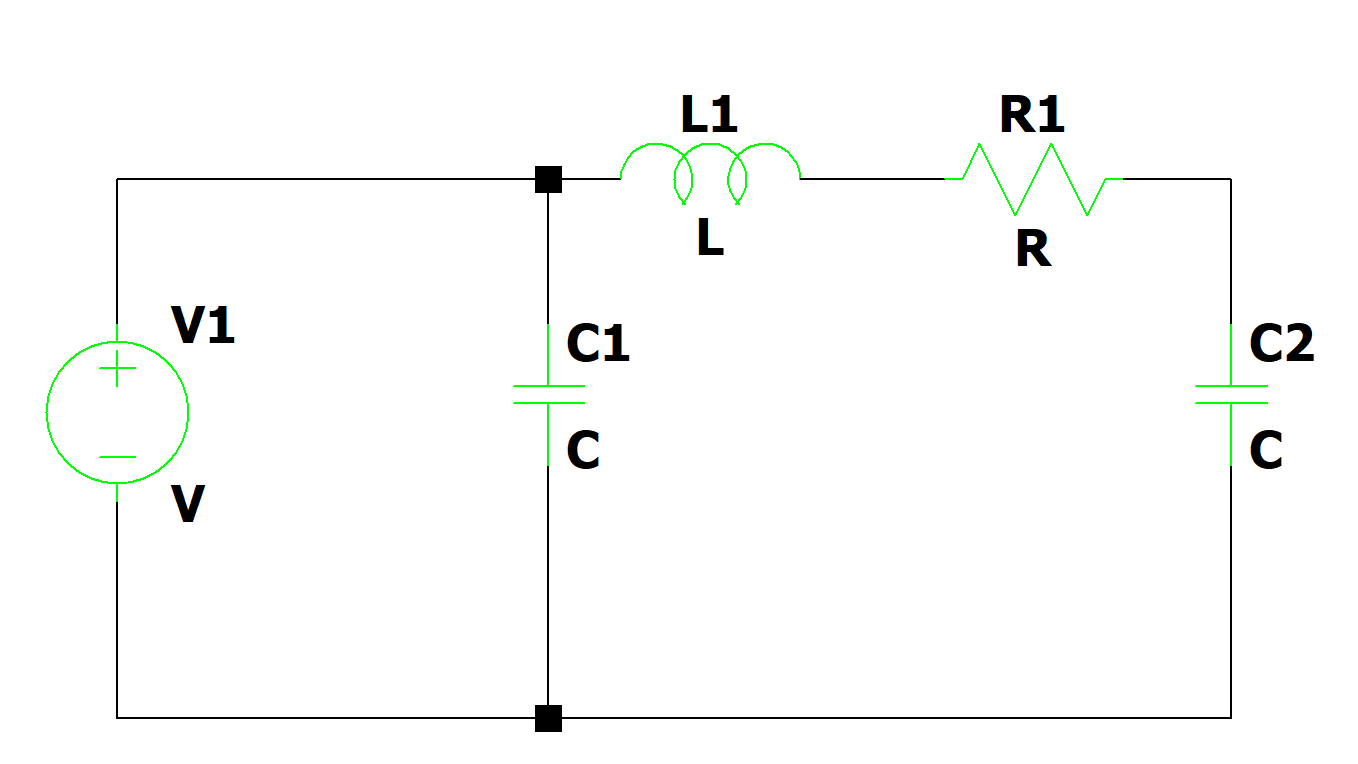
\includegraphics[width=0.7\textwidth]{IMG/data/overzicht/elektrischmodel_kabel.png}
\caption{Elektrisch model kabels}
\label{fig:elektrischmodel}
\end{figure}

In formule \ref{eq:30} wordt de capacitieve reactantie (\(X_c\)) berekend met behulp van de opgegeven formule, waarbij de capaciteit terug te vinden is in tabel \ref{tab:Kavel VI - Kabel data} en tabel \ref{tab:Kavel VII - Kabel data}.

% Vergelijking 30: Berekening van Xc
\begin{equation} \label{eq:30}
X_c = \frac{1}{{100 \times \pi \times \text{{Capaciteit}}}}
\end{equation}
\myequations{Berekening: Xc}

In formule \ref{eq:31} wordt de inductieve reactantie (\(X_l\)) berekend met behulp van de opgegeven formule, waarbij de inductantie terug te vinden is in tabel \ref{tab:Kavel VI - Kabel data} en tabel \ref{tab:Kavel VII - Kabel data}.
% Vergelijking 31: Berekening van Xl
\begin{equation} \label{eq:31}
X_l = 100 \times \pi \times \text{{Inductie}}
\end{equation}
\myequations{Berekening: Xl}

In formule \ref{eq:32} wordt de impedantie (\(Z\)) met behulp van de capacitieve reactantie (\(X_c\)), inductieve reactantie (\(X_l\)) en weerstand (\(R\)).
% Vergelijking 32: Berekening van Impedantie
\begin{equation} \label{eq:32}
Z = \sqrt{{(X_c - X_l)^2 + R^2}}
\end{equation}
\myequations{Berekening: Z}


In formule \ref{eq:33} worden de verliezen met behulp van de fase-spanning (\(\text{{Vfase}}\)) en impedantie (\(Z\)).
% Vergelijking 33: Berekening van Verliezen
\begin{equation} \label{eq:33}
\text{{Verliezen}} = \frac{{\text{{Vfase}}}}{{Z}}
\end{equation}
\myequations{Berekening: Verliezen}


In formule \ref{eq:34} wordt de fase-spanning (\(\text{{Vfase}}\)) met behulp van de opgegeven formule.
% Vergelijking 34: Berekening van Vfase
\begin{equation} \label{eq:34}
\text{{Vfase}} = \frac{{66000}}{{\sqrt{3}}}
\end{equation}
\myequations{Berekening: Vfase}


In formule \ref{eq:35} wordt de stroom per kabel met behulp van het vermogen per turbine, het aantal turbines en de fase-spanning.

% Vergelijking 35: Berekening van Stroom per kabel
\begin{equation} \label{eq:35}
\text{{Stroom per kabel}} = \frac{{\text{{Vermogen per turbine}} \times \text{{Aantal turbines}}}}{{\frac{{66000}}{{\sqrt{3}}}}} = \frac{{18000000 \times \text{{nTurbines}}}}{{\frac{{66000}}{{\sqrt{3}}}}}
\end{equation}
\myequations{Berekening: Stroom per kabel}

In formule \ref{eq:36} wordt de netto stroom door de verliezen af te trekken van de stroom per kabel.
% Vergelijking 36: Berekening van Netto stroom
\begin{equation} \label{eq:36}
\text{{Netto stroom}} = \text{{Stroom per kabel}} - \text{{Verliezen}}
\end{equation}
\myequations{Berekening: Netto stroom}


Met behulp van formule \ref{eq:30}, \ref{eq:31}, \ref{eq:32}, \ref{eq:33}, \ref{eq:34}, \ref{eq:35} en \ref{eq:36} kan tabel \ref{tab:Kavel VI - Kabel extra data} en tabel \ref{tab:Kavel VII - Kabel extra data} worden ingevuld.

\begin{table}[h]
\resizebox{\textwidth}{!}{
\begin{tabular}{|lrrrrrrrrrrrrrr|}
\hline
\rowcolor[HTML]{9B9B9B} 
\multicolumn{14}{|c|}{\cellcolor[HTML]{9B9B9B}\textbf{Kavel VI}} \\ \hline
\rowcolor[HTML]{C0C0C0} 
\multicolumn{1}{|l|}{\cellcolor[HTML]{C0C0C0}\textit{\textbf{Kabel nummer}}} &
  \multicolumn{1}{l|}{\cellcolor[HTML]{C0C0C0}\textit{\textbf{1}}} &
  \multicolumn{1}{l|}{\cellcolor[HTML]{C0C0C0}\textit{\textbf{2}}} &
  \multicolumn{1}{l|}{\cellcolor[HTML]{C0C0C0}\textit{\textbf{3}}} &
  \multicolumn{1}{l|}{\cellcolor[HTML]{C0C0C0}\textit{\textbf{4}}} &
  \multicolumn{1}{l|}{\cellcolor[HTML]{C0C0C0}\textit{\textbf{5}}} &
  \multicolumn{1}{l|}{\cellcolor[HTML]{C0C0C0}\textit{\textbf{6}}} &
  \multicolumn{1}{l|}{\cellcolor[HTML]{C0C0C0}\textit{\textbf{7}}} &
  \multicolumn{1}{l|}{\cellcolor[HTML]{C0C0C0}\textit{\textbf{8}}} &
  \multicolumn{1}{l|}{\cellcolor[HTML]{C0C0C0}\textit{\textbf{9}}} &
  \multicolumn{1}{l|}{\cellcolor[HTML]{C0C0C0}\textit{\textbf{10}}} &
  \multicolumn{1}{l|}{\cellcolor[HTML]{C0C0C0}\textit{\textbf{11}}} &
  \multicolumn{1}{l|}{\cellcolor[HTML]{C0C0C0}\textit{\textbf{12}}} &
  \textit{\textbf{13}} \\ \hline
\rowcolor[HTML]{FFFFFF} 
\multicolumn{1}{|l|}{\cellcolor[HTML]{A5A5A5}{\color[HTML]{FFFFFF} \textbf{Totaal (KM)}}} &
  \multicolumn{1}{l|}{\cellcolor[HTML]{FFFFFF}5,35} &
  \multicolumn{1}{l|}{\cellcolor[HTML]{FFFFFF}5,30} &
  \multicolumn{1}{l|}{\cellcolor[HTML]{FFFFFF}1,27} &
  \multicolumn{1}{l|}{\cellcolor[HTML]{FFFFFF}13,60} &
  \multicolumn{1}{l|}{\cellcolor[HTML]{FFFFFF}8,23} &
  \multicolumn{1}{l|}{\cellcolor[HTML]{FFFFFF}14,00} &
  \multicolumn{1}{l|}{\cellcolor[HTML]{FFFFFF}3,63} &
  \multicolumn{1}{l|}{\cellcolor[HTML]{FFFFFF}7,18} &
  \multicolumn{1}{l|}{\cellcolor[HTML]{FFFFFF}8,03} &
  \multicolumn{1}{l|}{\cellcolor[HTML]{FFFFFF}10,91} &
  \multicolumn{1}{l|}{\cellcolor[HTML]{FFFFFF}6,84} &
  \multicolumn{1}{l|}{\cellcolor[HTML]{FFFFFF}3,72} &
  5,88 \\ \hline
\rowcolor[HTML]{C0C0C0} 
\multicolumn{1}{|l|}{\cellcolor[HTML]{A5A5A5}{\color[HTML]{FFFFFF} \textbf{Weerstand (\(\Omega\))}}} &
  \multicolumn{1}{l|}{\cellcolor[HTML]{C0C0C0}0,09} &
  \multicolumn{1}{l|}{\cellcolor[HTML]{C0C0C0}0,09} &
  \multicolumn{1}{l|}{\cellcolor[HTML]{C0C0C0}0,02} &
  \multicolumn{1}{l|}{\cellcolor[HTML]{C0C0C0}0,24} &
  \multicolumn{1}{l|}{\cellcolor[HTML]{C0C0C0}0,14} &
  \multicolumn{1}{l|}{\cellcolor[HTML]{C0C0C0}0,25} &
  \multicolumn{1}{l|}{\cellcolor[HTML]{C0C0C0}0,06} &
  \multicolumn{1}{l|}{\cellcolor[HTML]{C0C0C0}0,13} &
  \multicolumn{1}{l|}{\cellcolor[HTML]{C0C0C0}0,14} &
  \multicolumn{1}{l|}{\cellcolor[HTML]{C0C0C0}0,19} &
  \multicolumn{1}{l|}{\cellcolor[HTML]{C0C0C0}0,12} &
  \multicolumn{1}{l|}{\cellcolor[HTML]{C0C0C0}0,07} &
  0,10 \\ \hline
\rowcolor[HTML]{FFFFFF} 
\multicolumn{1}{|l|}{\cellcolor[HTML]{A5A5A5}{\color[HTML]{FFFFFF} \textbf{Capaciteit (uF)}}} &
  \multicolumn{1}{l|}{\cellcolor[HTML]{FFFFFF}2,03} &
  \multicolumn{1}{l|}{\cellcolor[HTML]{FFFFFF}2,01} &
  \multicolumn{1}{l|}{\cellcolor[HTML]{FFFFFF}0,48} &
  \multicolumn{1}{l|}{\cellcolor[HTML]{FFFFFF}5,17} &
  \multicolumn{1}{l|}{\cellcolor[HTML]{FFFFFF}3,13} &
  \multicolumn{1}{l|}{\cellcolor[HTML]{FFFFFF}5,32} &
  \multicolumn{1}{l|}{\cellcolor[HTML]{FFFFFF}1,38} &
  \multicolumn{1}{l|}{\cellcolor[HTML]{FFFFFF}2,73} &
  \multicolumn{1}{l|}{\cellcolor[HTML]{FFFFFF}3,05} &
  \multicolumn{1}{l|}{\cellcolor[HTML]{FFFFFF}4,15} &
  \multicolumn{1}{l|}{\cellcolor[HTML]{FFFFFF}2,60} &
  \multicolumn{1}{l|}{\cellcolor[HTML]{FFFFFF}1,42} &
  2,24 \\ \hline
\rowcolor[HTML]{C0C0C0} 
\multicolumn{1}{|l|}{\cellcolor[HTML]{A5A5A5}{\color[HTML]{FFFFFF} \textbf{Inductie (mH)}}} &
  \multicolumn{1}{l|}{\cellcolor[HTML]{C0C0C0}1,66} &
  \multicolumn{1}{l|}{\cellcolor[HTML]{C0C0C0}1,64} &
  \multicolumn{1}{l|}{\cellcolor[HTML]{C0C0C0}0,39} &
  \multicolumn{1}{l|}{\cellcolor[HTML]{C0C0C0}4,22} &
  \multicolumn{1}{l|}{\cellcolor[HTML]{C0C0C0}2,55} &
  \multicolumn{1}{l|}{\cellcolor[HTML]{C0C0C0}4,34} &
  \multicolumn{1}{l|}{\cellcolor[HTML]{C0C0C0}1,12} &
  \multicolumn{1}{l|}{\cellcolor[HTML]{C0C0C0}2,22} &
  \multicolumn{1}{l|}{\cellcolor[HTML]{C0C0C0}2,49} &
  \multicolumn{1}{l|}{\cellcolor[HTML]{C0C0C0}3,38} &
  \multicolumn{1}{l|}{\cellcolor[HTML]{C0C0C0}2,12} &
  \multicolumn{1}{l|}{\cellcolor[HTML]{C0C0C0}1,15} &
  1,82 \\ \hline
\rowcolor[HTML]{C0C0C0} 
\multicolumn{1}{|l|}{\cellcolor[HTML]{A5A5A5}{\color[HTML]{FFFFFF} \textbf{Xc (\(\Omega\))}}} &
  \multicolumn{1}{l|}{\cellcolor[HTML]{C0C0C0}1565,715131} &
  \multicolumn{1}{l|}{\cellcolor[HTML]{C0C0C0}1581,679749} &
  \multicolumn{1}{l|}{\cellcolor[HTML]{C0C0C0}6585,358453} &
  \multicolumn{1}{l|}{\cellcolor[HTML]{C0C0C0}615,7888666} &
  \multicolumn{1}{l|}{\cellcolor[HTML]{C0C0C0}1017,315515} &
  \multicolumn{1}{l|}{\cellcolor[HTML]{C0C0C0}598,1986683} &
  \multicolumn{1}{l|}{\cellcolor[HTML]{C0C0C0}2309,505363} &
  \multicolumn{1}{l|}{\cellcolor[HTML]{C0C0C0}1167,141696} &
  \multicolumn{1}{l|}{\cellcolor[HTML]{C0C0C0}1042,640771} &
  \multicolumn{1}{l|}{\cellcolor[HTML]{C0C0C0}767,7184449} &
  \multicolumn{1}{l|}{\cellcolor[HTML]{C0C0C0}1225,541471} &
  \multicolumn{1}{l|}{\cellcolor[HTML]{C0C0C0}2249,349074} &
  1423,619298 \\ \hline
\rowcolor[HTML]{FFFFFF} 
\multicolumn{1}{|l|}{\cellcolor[HTML]{A5A5A5}{\color[HTML]{FFFFFF} \textbf{Xl (\(\Omega\))}}} &
  \multicolumn{1}{l|}{\cellcolor[HTML]{FFFFFF}0,521033142} &
  \multicolumn{1}{l|}{\cellcolor[HTML]{FFFFFF}0,515774115} &
  \multicolumn{1}{l|}{\cellcolor[HTML]{FFFFFF}0,123879282} &
  \multicolumn{1}{l|}{\cellcolor[HTML]{FFFFFF}1,324787631} &
  \multicolumn{1}{l|}{\cellcolor[HTML]{FFFFFF}0,801904091} &
  \multicolumn{1}{l|}{\cellcolor[HTML]{FFFFFF}1,36374338} &
  \multicolumn{1}{l|}{\cellcolor[HTML]{FFFFFF}0,353231253} &
  \multicolumn{1}{l|}{\cellcolor[HTML]{FFFFFF}0,698963525} &
  \multicolumn{1}{l|}{\cellcolor[HTML]{FFFFFF}0,782426217} &
  \multicolumn{1}{l|}{\cellcolor[HTML]{FFFFFF}1,062615441} &
  \multicolumn{1}{l|}{\cellcolor[HTML]{FFFFFF}0,665656359} &
  \multicolumn{1}{l|}{\cellcolor[HTML]{FFFFFF}0,362678022} &
  0,573039066 \\ \hline
\rowcolor[HTML]{C0C0C0} 
\multicolumn{1}{|l|}{\cellcolor[HTML]{A5A5A5}{\color[HTML]{FFFFFF} \textbf{Z (\(\Omega\))}}} &
  \multicolumn{1}{l|}{\cellcolor[HTML]{C0C0C0}1565,194101} &
  \multicolumn{1}{l|}{\cellcolor[HTML]{C0C0C0}1581,163978} &
  \multicolumn{1}{l|}{\cellcolor[HTML]{C0C0C0}6585,234574} &
  \multicolumn{1}{l|}{\cellcolor[HTML]{C0C0C0}614,4641251} &
  \multicolumn{1}{l|}{\cellcolor[HTML]{C0C0C0}1016,513621} &
  \multicolumn{1}{l|}{\cellcolor[HTML]{C0C0C0}596,8349752} &
  \multicolumn{1}{l|}{\cellcolor[HTML]{C0C0C0}2309,152133} &
  \multicolumn{1}{l|}{\cellcolor[HTML]{C0C0C0}1166,442739} &
  \multicolumn{1}{l|}{\cellcolor[HTML]{C0C0C0}1041,858354} &
  \multicolumn{1}{l|}{\cellcolor[HTML]{C0C0C0}766,6558532} &
  \multicolumn{1}{l|}{\cellcolor[HTML]{C0C0C0}1224,87582} &
  \multicolumn{1}{l|}{\cellcolor[HTML]{C0C0C0}2248,986397} &
  1423,046263 \\ \hline
\end{tabular}
}
\caption{Kabeldata van kavel VI}
\label{tab:Kavel VI - Kabel extra data}
\end{table}



\begin{table}[h]
\resizebox{\textwidth}{!}{
\begin{tabular}{|lrrrrrrrrrrrrrr|}
\hline
\rowcolor[HTML]{9B9B9B} 
\multicolumn{15}{|c|}{\cellcolor[HTML]{9B9B9B}\textbf{Kavel VII}} \\ \hline
\rowcolor[HTML]{C0C0C0} 
\multicolumn{1}{|l|}{\cellcolor[HTML]{C0C0C0}\textit{\textbf{Kabel nummer}}} &
  \multicolumn{1}{l|}{\cellcolor[HTML]{C0C0C0}\textit{\textbf{1}}} &
  \multicolumn{1}{l|}{\cellcolor[HTML]{C0C0C0}\textit{\textbf{2}}} &
  \multicolumn{1}{l|}{\cellcolor[HTML]{C0C0C0}\textit{\textbf{3}}} &
  \multicolumn{1}{l|}{\cellcolor[HTML]{C0C0C0}\textit{\textbf{4}}} &
  \multicolumn{1}{l|}{\cellcolor[HTML]{C0C0C0}\textit{\textbf{5}}} &
  \multicolumn{1}{l|}{\cellcolor[HTML]{C0C0C0}\textit{\textbf{6}}} &
  \multicolumn{1}{l|}{\cellcolor[HTML]{C0C0C0}\textit{\textbf{7}}} &
  \multicolumn{1}{l|}{\cellcolor[HTML]{C0C0C0}\textit{\textbf{8}}} &
  \multicolumn{1}{l|}{\cellcolor[HTML]{C0C0C0}\textit{\textbf{9}}} &
  \multicolumn{1}{l|}{\cellcolor[HTML]{C0C0C0}\textit{\textbf{10}}} &
  \multicolumn{1}{l|}{\cellcolor[HTML]{C0C0C0}\textit{\textbf{11}}} &
  \multicolumn{1}{l|}{\cellcolor[HTML]{C0C0C0}\textit{\textbf{12}}} &
  \multicolumn{1}{l|}{\cellcolor[HTML]{C0C0C0}\textit{\textbf{13}}} &
  \multicolumn{1}{l|}{\cellcolor[HTML]{C0C0C0}\textit{\textbf{14}}} \\ \hline
\rowcolor[HTML]{FFFFFF} 
\multicolumn{1}{|l|}{\cellcolor[HTML]{A5A5A5}{\color[HTML]{FFFFFF} \textbf{Totaal (KM)}}} &
  \multicolumn{1}{r|}{\cellcolor[HTML]{FFFFFF}6,27} &
  \multicolumn{1}{r|}{\cellcolor[HTML]{FFFFFF}4,95} &
  \multicolumn{1}{r|}{\cellcolor[HTML]{FFFFFF}5,81} &
  \multicolumn{1}{r|}{\cellcolor[HTML]{FFFFFF}7,92} &
  \multicolumn{1}{r|}{\cellcolor[HTML]{FFFFFF}9,08} &
  \multicolumn{1}{r|}{\cellcolor[HTML]{FFFFFF}14,13} &
  \multicolumn{1}{r|}{\cellcolor[HTML]{FFFFFF}8,61} &
  \multicolumn{1}{r|}{\cellcolor[HTML]{FFFFFF}8,61} &
  \multicolumn{1}{r|}{\cellcolor[HTML]{FFFFFF}5,46} &
  \multicolumn{1}{r|}{\cellcolor[HTML]{FFFFFF}9,18} &
  \multicolumn{1}{r|}{\cellcolor[HTML]{FFFFFF}8,21} &
  \multicolumn{1}{r|}{\cellcolor[HTML]{FFFFFF}9,02} &
  \multicolumn{1}{r|}{\cellcolor[HTML]{FFFFFF}3,82} &
  1,13 \\ \hline
\rowcolor[HTML]{C0C0C0} 
\multicolumn{1}{|l|}{\cellcolor[HTML]{A5A5A5}{\color[HTML]{FFFFFF} \textbf{Weerstand (\(\Omega\))}}} &
  \multicolumn{1}{r|}{\cellcolor[HTML]{C0C0C0}0,11} &
  \multicolumn{1}{r|}{\cellcolor[HTML]{C0C0C0}0,09} &
  \multicolumn{1}{r|}{\cellcolor[HTML]{C0C0C0}0,10} &
  \multicolumn{1}{r|}{\cellcolor[HTML]{C0C0C0}0,14} &
  \multicolumn{1}{r|}{\cellcolor[HTML]{C0C0C0}0,16} &
  \multicolumn{1}{r|}{\cellcolor[HTML]{C0C0C0}0,25} &
  \multicolumn{1}{r|}{\cellcolor[HTML]{C0C0C0}0,15} &
  \multicolumn{1}{r|}{\cellcolor[HTML]{C0C0C0}0,15} &
  \multicolumn{1}{r|}{\cellcolor[HTML]{C0C0C0}0,10} &
  \multicolumn{1}{r|}{\cellcolor[HTML]{C0C0C0}0,16} &
  \multicolumn{1}{r|}{\cellcolor[HTML]{C0C0C0}0,14} &
  \multicolumn{1}{r|}{\cellcolor[HTML]{C0C0C0}0,16} &
  \multicolumn{1}{r|}{\cellcolor[HTML]{C0C0C0}0,07} &
  0,02 \\ \hline
\rowcolor[HTML]{FFFFFF} 
\multicolumn{1}{|l|}{\cellcolor[HTML]{A5A5A5}{\color[HTML]{FFFFFF} \textbf{Capaciteit (uF)}}} &
  \multicolumn{1}{r|}{\cellcolor[HTML]{FFFFFF}2,38} &
  \multicolumn{1}{r|}{\cellcolor[HTML]{FFFFFF}1,88} &
  \multicolumn{1}{r|}{\cellcolor[HTML]{FFFFFF}2,21} &
  \multicolumn{1}{r|}{\cellcolor[HTML]{FFFFFF}3,01} &
  \multicolumn{1}{r|}{\cellcolor[HTML]{FFFFFF}3,45} &
  \multicolumn{1}{r|}{\cellcolor[HTML]{FFFFFF}5,37} &
  \multicolumn{1}{r|}{\cellcolor[HTML]{FFFFFF}3,27} &
  \multicolumn{1}{r|}{\cellcolor[HTML]{FFFFFF}3,27} &
  \multicolumn{1}{r|}{\cellcolor[HTML]{FFFFFF}2,08} &
  \multicolumn{1}{r|}{\cellcolor[HTML]{FFFFFF}3,49} &
  \multicolumn{1}{r|}{\cellcolor[HTML]{FFFFFF}3,12} &
  \multicolumn{1}{r|}{\cellcolor[HTML]{FFFFFF}3,43} &
  \multicolumn{1}{r|}{\cellcolor[HTML]{FFFFFF}1,45} &
  0,43 \\ \hline
\rowcolor[HTML]{C0C0C0} 
\multicolumn{1}{|l|}{\cellcolor[HTML]{A5A5A5}{\color[HTML]{FFFFFF} \textbf{Inductie (mH)}}} &
  \multicolumn{1}{r|}{\cellcolor[HTML]{C0C0C0}1,94} &
  \multicolumn{1}{r|}{\cellcolor[HTML]{C0C0C0}1,53} &
  \multicolumn{1}{r|}{\cellcolor[HTML]{C0C0C0}1,80} &
  \multicolumn{1}{r|}{\cellcolor[HTML]{C0C0C0}2,45} &
  \multicolumn{1}{r|}{\cellcolor[HTML]{C0C0C0}2,81} &
  \multicolumn{1}{r|}{\cellcolor[HTML]{C0C0C0}4,38} &
  \multicolumn{1}{r|}{\cellcolor[HTML]{C0C0C0}2,67} &
  \multicolumn{1}{r|}{\cellcolor[HTML]{C0C0C0}2,67} &
  \multicolumn{1}{r|}{\cellcolor[HTML]{C0C0C0}1,69} &
  \multicolumn{1}{r|}{\cellcolor[HTML]{C0C0C0}2,85} &
  \multicolumn{1}{r|}{\cellcolor[HTML]{C0C0C0}2,55} &
  \multicolumn{1}{r|}{\cellcolor[HTML]{C0C0C0}2,80} &
  \multicolumn{1}{r|}{\cellcolor[HTML]{C0C0C0}1,19} &
  0,35 \\ \hline
\rowcolor[HTML]{C0C0C0} 
\multicolumn{1}{|l|}{\cellcolor[HTML]{A5A5A5}{\color[HTML]{FFFFFF} \textbf{Xc (\(\Omega\))}}} &
  \multicolumn{1}{r|}{\cellcolor[HTML]{C0C0C0}1335,977026} &
  \multicolumn{1}{r|}{\cellcolor[HTML]{C0C0C0}1693,263787} &
  \multicolumn{1}{r|}{\cellcolor[HTML]{C0C0C0}1441,255326} &
  \multicolumn{1}{r|}{\cellcolor[HTML]{C0C0C0}1057,782037} &
  \multicolumn{1}{r|}{\cellcolor[HTML]{C0C0C0}922,5303912} &
  \multicolumn{1}{r|}{\cellcolor[HTML]{C0C0C0}592,9899442} &
  \multicolumn{1}{r|}{\cellcolor[HTML]{C0C0C0}973,0022014} &
  \multicolumn{1}{r|}{\cellcolor[HTML]{C0C0C0}973,0022014} &
  \multicolumn{1}{r|}{\cellcolor[HTML]{C0C0C0}1533,328931} &
  \multicolumn{1}{r|}{\cellcolor[HTML]{C0C0C0}912,5804502} &
  \multicolumn{1}{r|}{\cellcolor[HTML]{C0C0C0}1019,792543} &
  \multicolumn{1}{r|}{\cellcolor[HTML]{C0C0C0}928,564012} &
  \multicolumn{1}{r|}{\cellcolor[HTML]{C0C0C0}2191,100171} &
  7412,899073 \\ \hline
\rowcolor[HTML]{FFFFFF} 
\multicolumn{1}{|l|}{\cellcolor[HTML]{A5A5A5}{\color[HTML]{FFFFFF} \textbf{Xl (\(\Omega\))}}} &
  \multicolumn{1}{r|}{\cellcolor[HTML]{FFFFFF}0,610631364} &
  \multicolumn{1}{r|}{\cellcolor[HTML]{FFFFFF}0,481785225} &
  \multicolumn{1}{r|}{\cellcolor[HTML]{FFFFFF}0,566027032} &
  \multicolumn{1}{r|}{\cellcolor[HTML]{FFFFFF}0,771226439} &
  \multicolumn{1}{r|}{\cellcolor[HTML]{FFFFFF}0,8842955} &
  \multicolumn{1}{r|}{\cellcolor[HTML]{FFFFFF}1,375722273} &
  \multicolumn{1}{r|}{\cellcolor[HTML]{FFFFFF}0,838425106} &
  \multicolumn{1}{r|}{\cellcolor[HTML]{FFFFFF}0,838425106} &
  \multicolumn{1}{r|}{\cellcolor[HTML]{FFFFFF}0,532038141} &
  \multicolumn{1}{r|}{\cellcolor[HTML]{FFFFFF}0,893937048} &
  \multicolumn{1}{r|}{\cellcolor[HTML]{FFFFFF}0,799956304} &
  \multicolumn{1}{r|}{\cellcolor[HTML]{FFFFFF}0,878549527} &
  \multicolumn{1}{r|}{\cellcolor[HTML]{FFFFFF}0,37231957} &
  0,110049991 \\ \hline
\rowcolor[HTML]{C0C0C0} 
\multicolumn{1}{|l|}{\cellcolor[HTML]{A5A5A5}{\color[HTML]{FFFFFF} \textbf{Z (\(\Omega\))}}} &
  \multicolumn{1}{r|}{\cellcolor[HTML]{C0C0C0}1335,366399} &
  \multicolumn{1}{r|}{\cellcolor[HTML]{C0C0C0}1692,782004} &
  \multicolumn{1}{r|}{\cellcolor[HTML]{C0C0C0}1440,689302} &
  \multicolumn{1}{r|}{\cellcolor[HTML]{C0C0C0}1057,01082} &
  \multicolumn{1}{r|}{\cellcolor[HTML]{C0C0C0}921,6461094} &
  \multicolumn{1}{r|}{\cellcolor[HTML]{C0C0C0}591,6142736} &
  \multicolumn{1}{r|}{\cellcolor[HTML]{C0C0C0}972,163788} &
  \multicolumn{1}{r|}{\cellcolor[HTML]{C0C0C0}972,163788} &
  \multicolumn{1}{r|}{\cellcolor[HTML]{C0C0C0}1532,796896} &
  \multicolumn{1}{r|}{\cellcolor[HTML]{C0C0C0}911,6865273} &
  \multicolumn{1}{r|}{\cellcolor[HTML]{C0C0C0}1018,992597} &
  \multicolumn{1}{r|}{\cellcolor[HTML]{C0C0C0}927,6854759} &
  \multicolumn{1}{r|}{\cellcolor[HTML]{C0C0C0}2190,727852} &
  7412,789023 \\ \hline
\end{tabular}
}
\caption{Kabeldata van kavel VII}
\label{tab:Kavel VII - Kabel extra data}
\end{table}

Er is voor deze kabel gekozen omdat dit een keuze was met een veilig marge voor de stroom die het kan weerstaan. Daarnaast is voor de kabel van ABB gekozen omdat bij toekomstige nieuwe inzichten er veel overige opties zijn voor alternatieve kabels om de meest optimale kabel te behouden voor de betreffende situatie. Ook biedt ABB veel informatie over de kabels wat ervoor zorgt dat zo accuraat mogelijke berekeningen kunnen worden gedaan. Hierdoor is het ontwerp van het windpark accuraat met de realiteit. 